\documentclass{article}
\usepackage[a3paper]{geometry}

\usepackage[active,tightpage]{preview}
\PreviewEnvironment{tikzpicture}

\usepackage{tikz}
\usetikzlibrary{positioning}
\usepackage{graphicx}

\begin{document}

\begin{preview}

\centering
\begin{tikzpicture}

%%%%-------------------------------------------------------------------------------------

\node[] (figure) at (3,10) {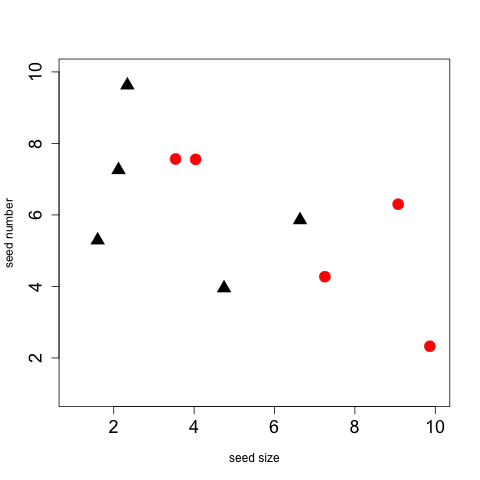
\includegraphics[width=.15\textwidth]{figure.png}};
\node[] (figure2) at (7,10) {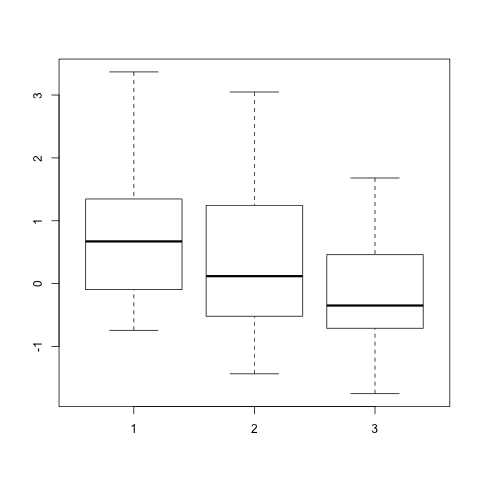
\includegraphics[width=.15\textwidth]{figure2.png}};

\node[] (figure_D) at (0,5) {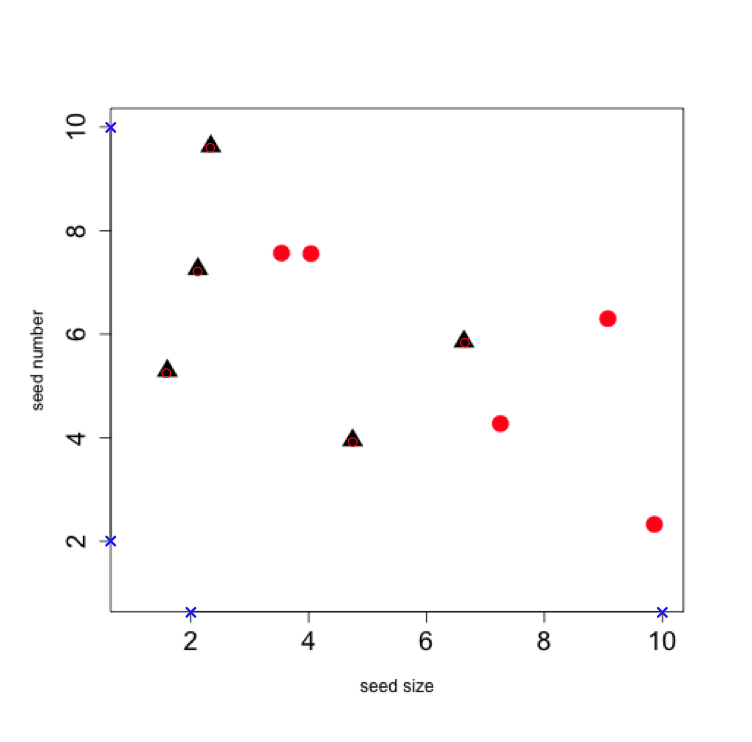
\includegraphics[width=.15\textwidth]{figure_digitize.png}};
\draw[->,thick, line width=0.3mm] (figure.south) -- (figure_D.north) ;

\node[] (figure2_D) at (3,5) {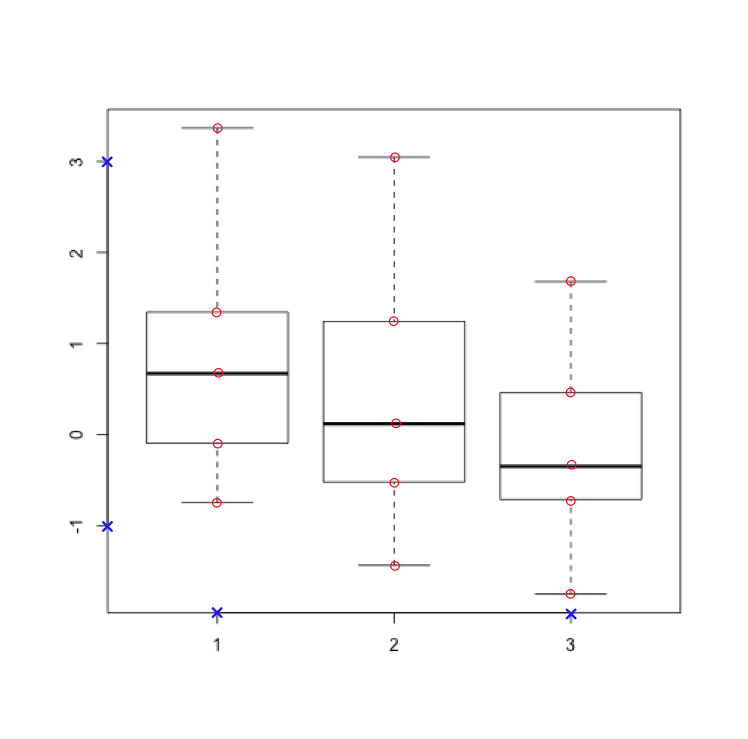
\includegraphics[width=.15\textwidth]{figure2_digitize.png}};
\draw[->,thick, line width=0.3mm] (figure2.south) -- (figure2_D.north) ;


\node[] (figure_mD) at (7,5) {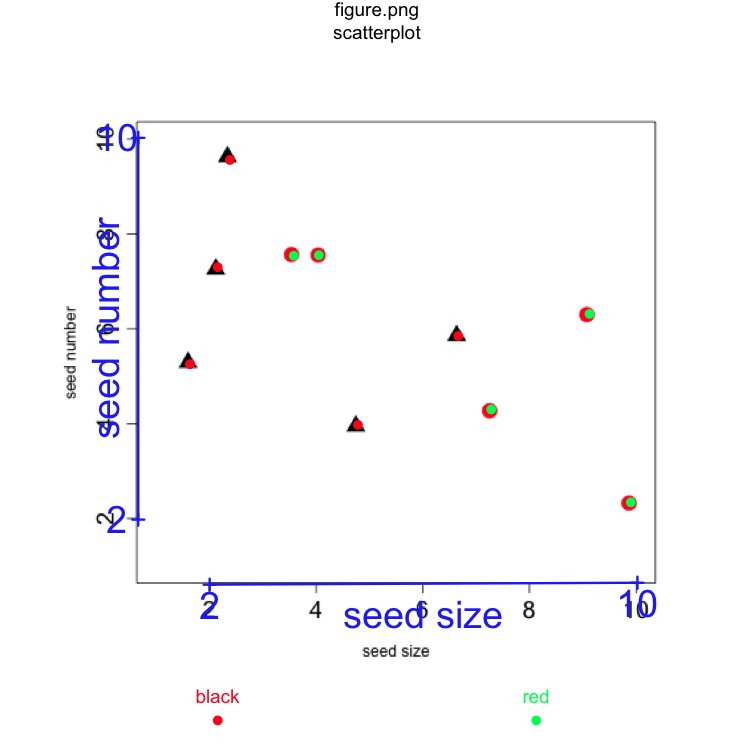
\includegraphics[width=.15\textwidth]{figure_metaDigitise.png}};
\draw[->,thick, line width=0.3mm] (figure.south) -- (figure_mD.north);

\node[] (figure2_mD) at (10,5) {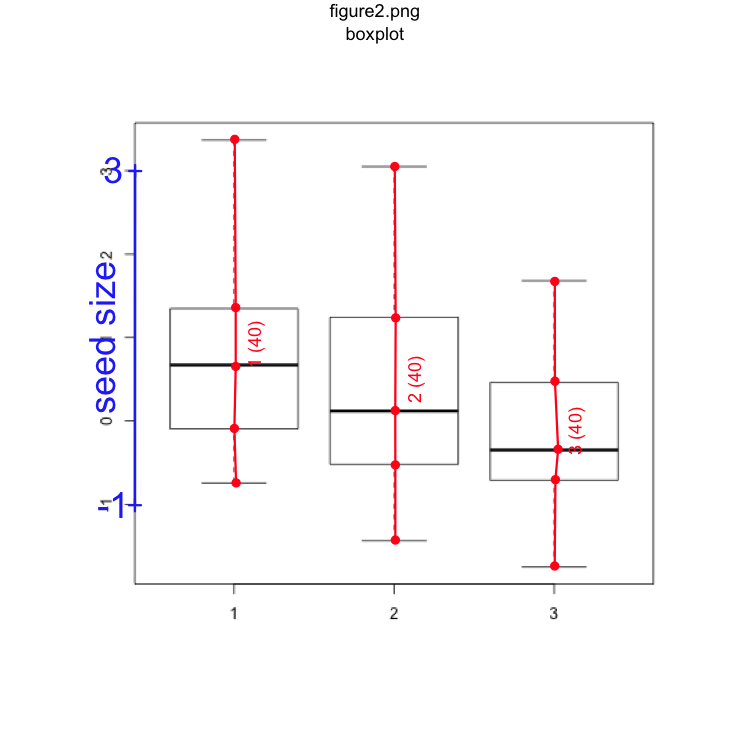
\includegraphics[width=.15\textwidth]{figure2_metaDigitise.png}};
\draw[->,thick, line width=0.3mm] (figure2.south) -- (figure2_mD.north);

\node[] (label_D) at (0,8) {digitize};
\node[] (label_D) at (10,8) {metaDigitise};


\setlength{\tabcolsep}{0.25em}
\node[inner sep=0pt, text width=2.5cm, anchor=north] (output_D) at (0,2) {\tiny   
\begin{tabular}{c c}
x & y\\
2.329895 & 9.605761\\
2.114273 & 7.212674\\
1.583472 & 5.246919\\
4.747202 & 3.914303\\
6.648952 & 5.837144\\
3.518762 & 7.556821\\
4.027756 & 7.544506\\
7.247960 & 4.248326\\
9.070899 & 6.302404\\
9.867233 & 2.323294\\
\end{tabular}
};

\node[inner sep=0pt, text width=2.5cm, anchor=north] (output2_D) at (3,2) {\tiny   
\begin{tabular}{c c}
x & y\\
1.00381 & 3.366921\\
1.00332 & 1.344158\\
1.00672 & 0.664347\\
1.00313 & -0.098183\\
0.99579 & -0.741522\\
2.00424 & 3.031860\\
2.00210 & 1.240030\\
2.01120 & 0.112484\\
1.99990 & -0.532548\\
2.00292 & -1.421841\\
2.99886 & 1.659290\\
2.99899 & 0.452495\\
3.01687 & -0.358099\\
2.99800 & -0.717574\\
2.99575 & -1.749286\\
\end{tabular}
};

\node[inner sep=0pt, anchor=north] (output_mD) at (8.5,2) {\tiny   
\begin{tabular}{c c c c c c c c}
filename & group\_id & variable & mean & sd & n & r & plot\_type\\
figure.png & black & seed size & 3.51610 & 2.12806 & 5 & -0.40887 & scatterplot\\
figure.png & black & seed number & 6.38350 & 2.12550 & 5 & -0.40887 & scatterplot\\
figure.png & red & seed size & 6.77229 & 2.87290 & 5 & -0.79541 & scatterplot\\
figure.png & red & seed number & 5.60961 & 2.24468 & 5 & -0.79541 & scatterplot\\
figure2.png & 1 & seed size & 0.81727 & 1.03320 & 40 & NA & boxplot\\
figure2.png & 2 & seed size & 0.41903 & 1.19537 & 40 & NA & boxplot\\
figure2.png & 3 & seed size & -0.14119 & 0.84790 & 40 & NA & boxplot\\
% filename & group\_id & variable & mean & sd & n & plot\_type\\
% figure2.png & 1 & seed size & 0.81727 & 1.03320 & 40 & boxplot\\
% figure2.png & 2 & seed size & 0.41903 & 1.19537 & 40 & boxplot\\
% figure2.png & 3 & seed size & -0.14119 & 0.84789 & 40 & boxplot\\
\end{tabular}
};





\draw[->,thick, line width=0.3mm] (figure_D) -- (output_D);
\draw[->,thick, line width=0.3mm] (figure2_D) -- (output2_D);
\draw[->,thick, line width=0.3mm] (figure_mD.south) -- (output_mD);
\draw[->,thick, line width=0.3mm] (figure2_mD.south) -- (output_mD);

\end{tikzpicture}

%\end{frame}
\end{preview}
\end{document}